\section{行为型模式}

\subsection{观察者模式}

\subsubsection{模式动机}
建立一种对象与对象之间的依赖关系,\textbf{一个对象发生改变时将自动通知其他对象,其他对象将相应做出反应}。
\begin{itemize}
    \item 发生改变的对象称为观察目标,而被通知的对象称为观察者。
    \item 一个观察目标可以对应多个观察者,而且这些观察者之间没有相互联系,可以根据需要增加和删除观察者,使得系统更易于扩展。
\end{itemize}

\subsubsection{模式定义}
观察者模式(Observer Pattern):定义对象间的一种一对多依赖关系,使得每当一个对象状态发生改变时,其相关依赖对象皆得到通知并被自动更新。观察者模式又叫做发布-订阅(Publish/Subscribe)模式、模型-视图 (Model/View)模式、源-监听器(Source/Listener) 模式或从属者(Dependents)模式。观察者模式是一种对象行为型模式。

\subsubsection{模式结构}
观察者模式包含如下角色:
\vspace{-0.8em}
\begin{multicols}{2}
    \begin{itemize}
        \item Subject:目标
        \item ConcreteSubject:具体目标
        \item Observer:观察者
        \item ConcreteObserver:具体观察者
    \end{itemize}
\end{multicols}
\vspace{-1em}

\begin{figure}[H]
    \vspace{-0.5em}
	\centering
	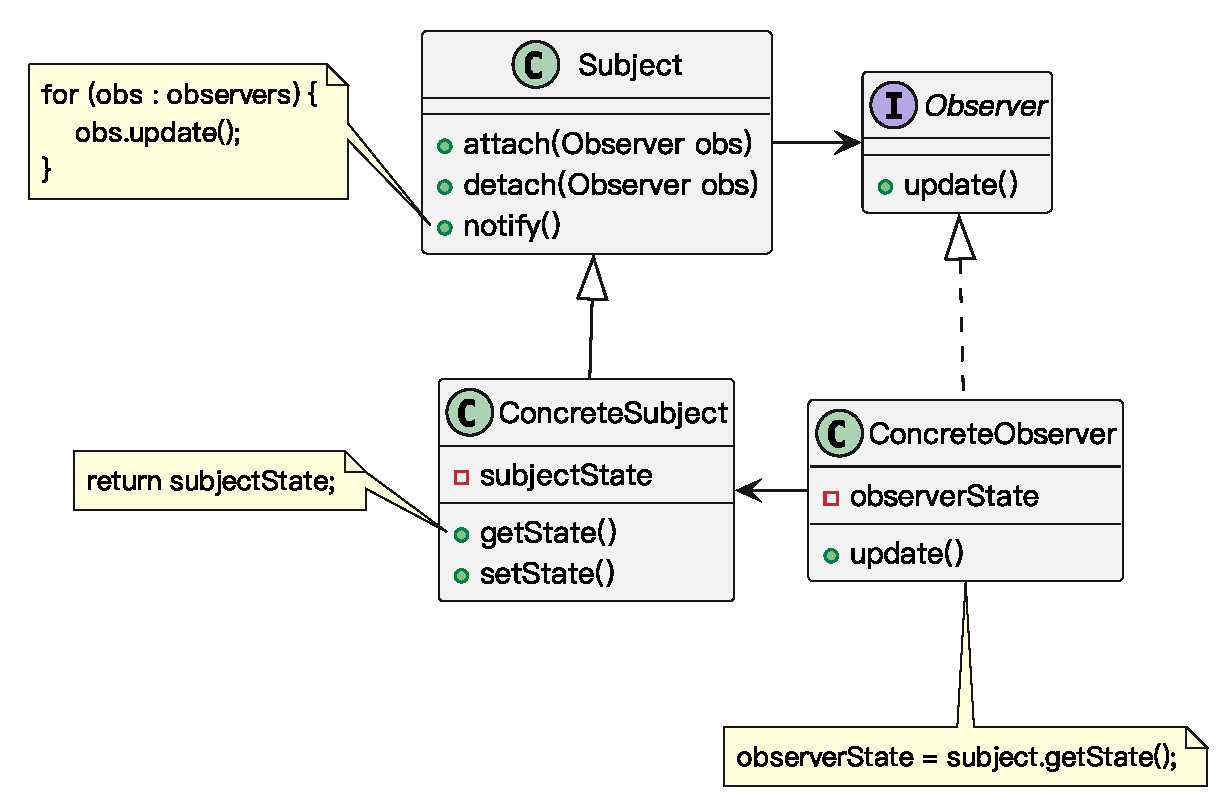
\includegraphics[width=0.7\textwidth]{images/观察者模式结构.eps}
    \vspace{-1em}
\end{figure}

\subsubsection{模式分析}
\begin{itemize}
    \item 观察者模式描述了\textbf{如何建立对象与对象之间的依赖关系},如何构造满足这种需求的系统。
    \item 这一模式中的关键对象是观察目标和观察者,\textbf{一个目标可以有任意数目的与之相依赖的观察者,一旦目标的状态发生改变,所有的观察者都将得到通知}。
    \item 作为对这个通知的响应,每个观察者都将即时更新自己的状态,以与目标状态同步,这种交互也称为\textbf{发布-订阅}(publish-subscribe)。目标是通知的发布者,它发出通知时并不需要知道谁是它的观察者,可以有任意数目的观察者订阅它并接收通知。
\end{itemize}

观察者模式顺序图如下所示:
\begin{figure}[H]
    \vspace{-0.5em}
	\centering
	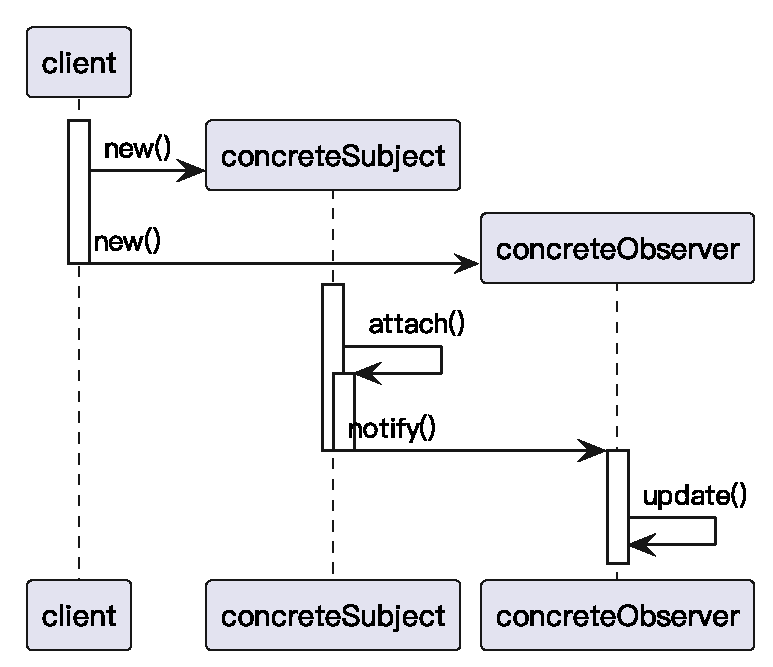
\includegraphics[width=0.45\textwidth]{images/观察者模式顺序图.eps}
    \vspace{-1em}
\end{figure}

观察者模式典型代码:
\begin{figure}[H]
    \vspace{-0.5em}
	\centering
	\includegraphics[width=0.95\textwidth]{images/观察者模式典型代码.pdf}
    \vspace{-1em}
\end{figure}

\subsubsection{模式实例}
猫、狗与老鼠:假设猫是老鼠和狗的观察目标,老鼠和狗是观察者,猫叫老鼠跑,狗也跟着叫,使用观察者模式描述该过程。
\begin{figure}[H]
    \vspace{-0.5em}
	\centering
	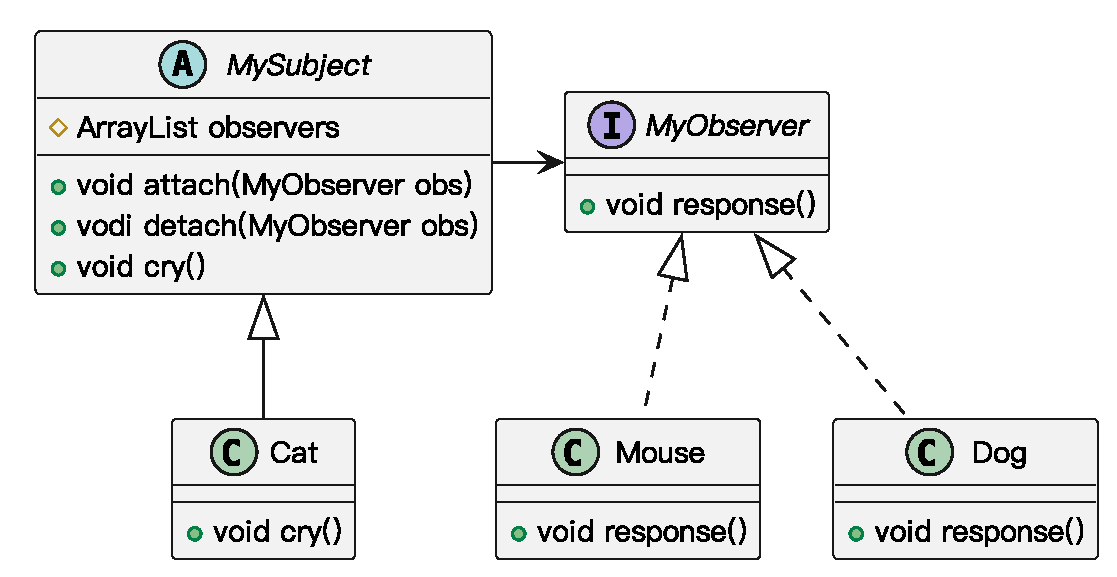
\includegraphics[width=0.6\textwidth]{images/观察者模式实例1.eps}
    \vspace{-1em}
\end{figure}

自定义登录控件:Java事件处理模型中应用了观察者模式,下面通过一个实例来学习如何自定义Java控件,并给该控件增加相应的事件。该实例基于Java Swing/AWT控件,在Swing/AWT的相关类中封装了对事件的底层处理。
\begin{figure}[H]
    \vspace{-0.5em}
	\centering
	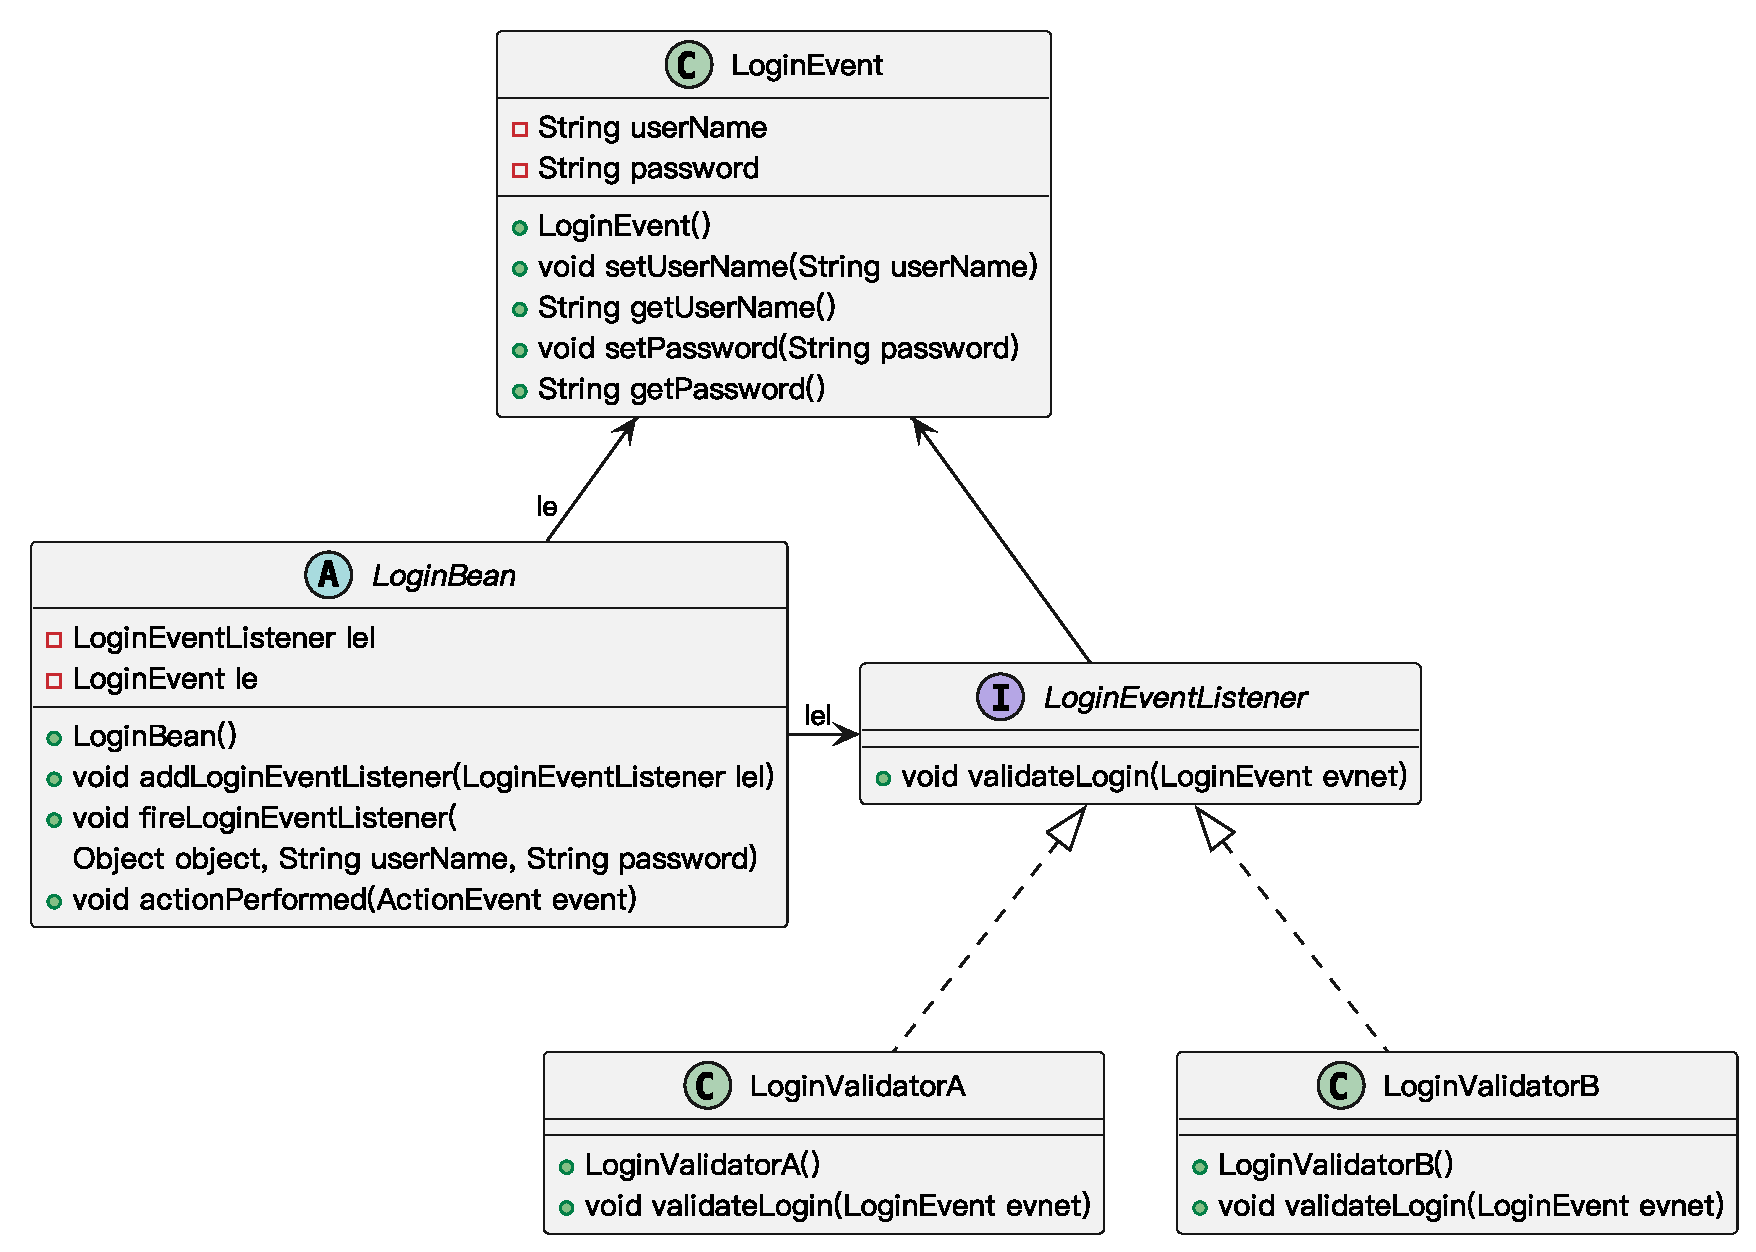
\includegraphics[width=0.85\textwidth]{images/观察者模式实例2.eps}
    \vspace{-1em}
\end{figure}

\subsubsection{模式优缺点}
观察者模式的优点:
\begin{itemize}
    \item 观察者模式可以\textbf{实现表示层和数据逻辑层的分离},并定义了稳定的消息更新传递机制,抽象了更新接口,使得可以有各种各样不同的表示层作为具体观察者角色。
    \item 观察者模式在观察目标和观察者之间\textbf{建立一个抽象的耦合}。
    \item 观察者模式\textbf{支持广播通信}。
    \item 观察者模式\textbf{符合开闭原则}的要求。
\end{itemize}

观察者模式的缺点:
\begin{itemize}
    \item 如果一个观察目标对象有很多直接和间接的观察者的话,\textbf{将所有的观察者都通知到会花费很多时间}。
    \item 如果在观察者和观察目标之间\textbf{有循环依赖}的话,观察目标会触发它们之间进行循环调用,\textbf{可能导致系统崩溃}。
    \item 观察者模式\textbf{没有相应的机制让观察者知道所观察的目标对象是怎么发生变化的},而仅仅只是知道观察目标发生了变化。
\end{itemize}

\subsubsection{模式适用环境}
在以下情况下可以使用观察者模式:
\begin{itemize}
    \item 一个抽象模型有两个方面,其中一个方面依赖于另一个方面。将这些方面封装在独立的对象中使它们可以各自独立地改变和复用。
    \item 一个对象的改变将导致其他一个或多个对象也发生改变,而不知道具体有多少对象将发生改变,可以降低对象之间的耦合度。
    \item 一个对象必须通知其他对象,而并不知道这些对象是谁。需要在系统中创建一个触发链,A对象的行为将影响B对象,B对象的行为将影响C对象……,可以使用观察者模式创建一种链式触发机制。
\end{itemize}

\subsubsection{模式应用}
\ding{172} JDK1.1版本及以后的各个版本中,事件处理模型采用基于观察者模式的委派事件模型(Delegation Event Model, DEM)。
\begin{itemize}
    \item 在DEM中,事件的发布者称为事件源(Event Source),而订阅者叫做事件监听器(Event Listener),在这个过程中还可以通过事件对象(Event Object)来传递与事件相关的信息,可以在事件监听者的实现类中实现事件处理,因此事件监听对象又可以称为事件处理对象。
    \item 事件源对象、事件监听对象(事件处理对象)和事件对象构成了Java事件处理模型的三要素。
\end{itemize}

\ding{173} 除了AWT中的事件处理之外,Java语言解析XML的技术SAX2以及Servlet技术的事件处理机制都基于DEM,它们都是观察者模式的应用。

\ding{174} 观察者模式在软件开发中应用非常广泛,如某电子商务网站可以在执行发送操作后给用户多个发送商品打折信息,某团队战斗游戏中某队友牺牲将给所有成员提示等等,\textbf{凡是涉及到一对一或者一对多的对象交互场景都可以使用观察者模式}。

\subsubsection{模式扩展}
\paragraph*{Java语言提供的对观察者模式的支持}~{} \par
在JDK的\sverb|java.util|\;包中,提供了\sverb|Observable|\;类以及\sverb|Observer|\;接口,它们构成了Java语言对观察者模式的支持。
\begin{figure}[H]
    \vspace{-0.5em}
	\centering
	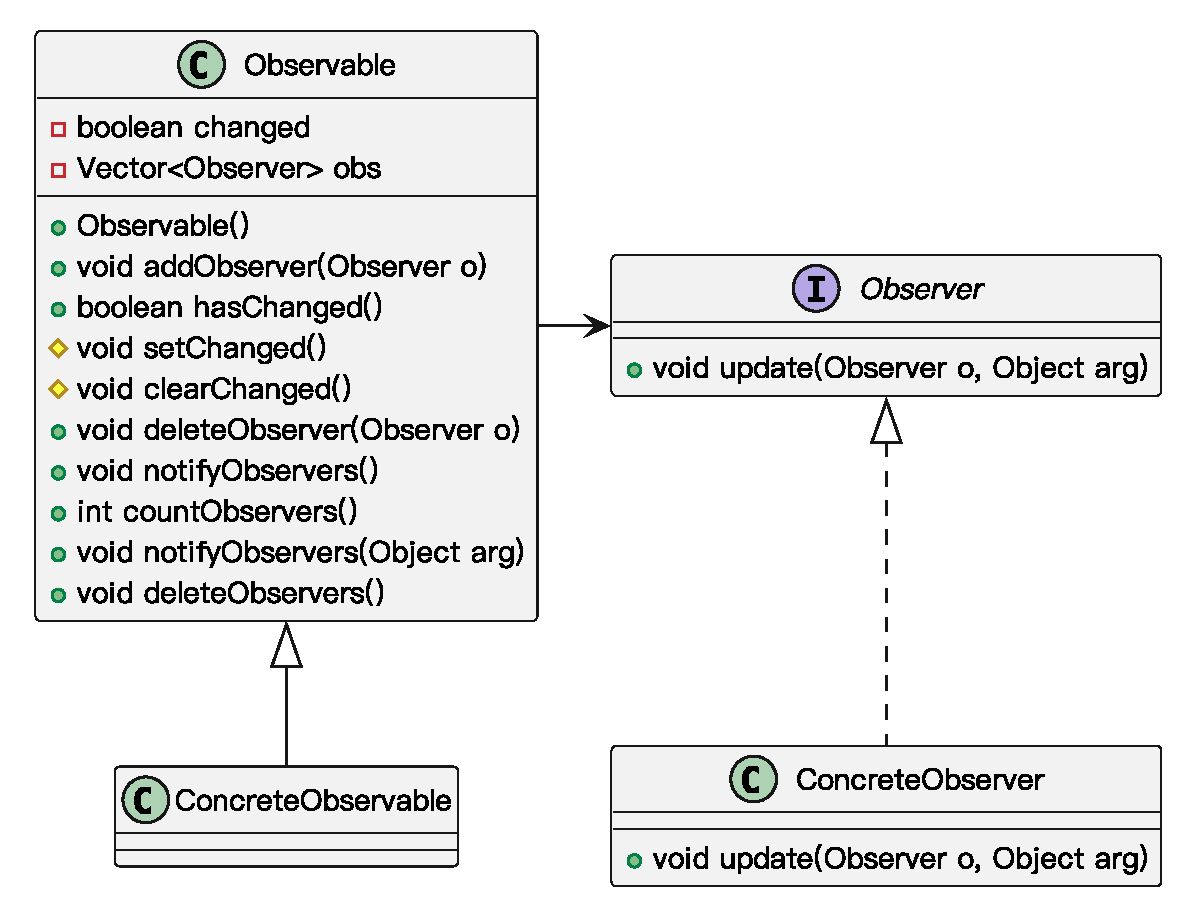
\includegraphics[width=0.68\textwidth]{images/观察者模式拓展1.eps}
    \vspace{-1em}
\end{figure}

\paragraph*{MVC模式}~{} \par
MVC模式是一种架构模式,它包含三个角色:模型(Model),视图(View)和控制器(Controller)。观察者模式可以用来实现MVC模式,观察者模式中的观察目标就是MVC模式中的模型(Model),而观察者就是MVC中的视图(View),控制器(Controller)充当两者之间的中介者(Mediator)。当模型层的数据发生改变时,视图层将自动改变其显示内容。
\begin{figure}[H]
    \vspace{-0.5em}
	\centering
	\includegraphics[width=0.45\textwidth]{images/观察者模式拓展2.pdf}
    \vspace{-1em}
\end{figure}


\subsection{中介者模式}

\subsubsection{模式动机}
在用户与用户直接聊天的设计方案中,用户对象之间存在很强的关联性,将导致系统出现如下问题:
\begin{itemize}
    \item \textbf{系统结构复杂}:对象之间存在大量的相互关联和调用,若有一个对象发生变化,则需要跟踪和该对象关联的其他所有对象,并进行适当处理。
    \item \textbf{对象可重用性差}:由于一个对象和其他对象具有很强的关联,若没有其他对象的支持,一个对象很难被另一个系统或模块重用,这些对象表现出来更像一个不可分割的整体,职责较为混乱。
    \item \textbf{系统扩展性低}:增加一个新的对象需要在原有相关对象上增加引用,增加新的引用关系也需要调整原有对象,系统耦合度很高,对象操作很不灵活,扩展性差。
\end{itemize}

在面向对象的软件设计与开发过程中,根据“单一职责原则”,我们应该尽量将对象细化,使其只负责或呈现单一的职责。

对于一个模块,可能由很多对象构成,而且这些对象之间可能存在相互的引用,\textbf{为了减少对象两两之间复杂的引用关系,使之成为一个松耦合的系统,我们需要使用中介者模式},这就是中介者模式的模式动机。

\subsubsection{模式定义}
中介者模式(Mediator Pattern)定义:用一个中介对象来封装一系列的对象交互,中介者使各对象不需要显式地相互引用,从而使其耦合松散,而且可以独立地改变它们之间的交互。中介者模式又称为调停者模式,它是一种对象行为型模式。

\subsubsection{模式结构}
中介者模式包含如下角色:
\vspace{-0.8em}
\begin{multicols}{2}
    \begin{itemize}
        \item Mediator:抽象中介者
        \item ConcreteMediator:具体中介者
        \item Colleague:抽象同事类
        \item ConcreteColleague:具体同事类
    \end{itemize}
\end{multicols}
\vspace{-1em}

\begin{figure}[H]
    \vspace{-0.5em}
	\centering
	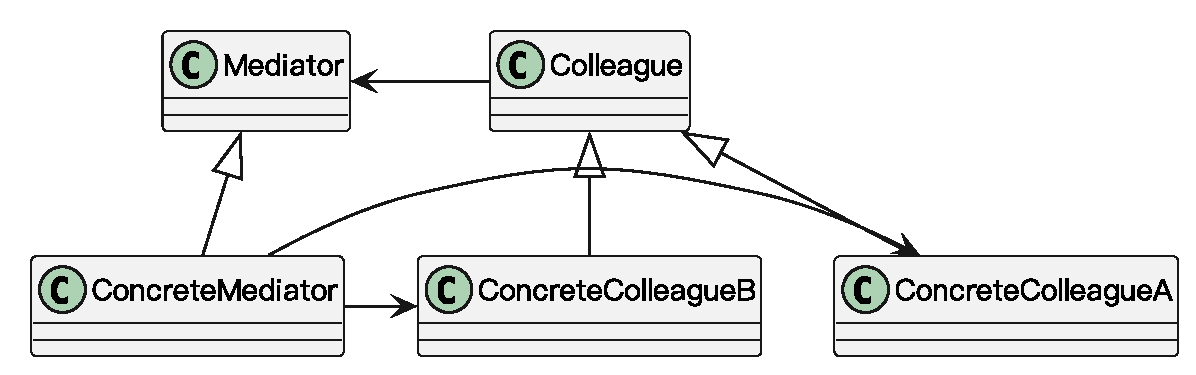
\includegraphics[width=0.7\textwidth]{images/中介者模式结构.eps}
    \vspace{-1em}
\end{figure}

\subsubsection{模式分析}
中介者模式可以使对象之间的关系数量急剧减少:
\begin{figure}[H]
    \vspace{-0.5em}
	\centering
	\includegraphics[width=0.68\textwidth]{images/中介者模式分析.pdf}
    \vspace{-1em}
\end{figure}

中介者承担两方面的职责:
\begin{itemize}
    \item \textbf{中转作用(结构性)}:通过中介者提供的中转作用,各个同事对象就不再需要显式引用其他同事,当需要和其他同事进行通信时,通过中介者即可。该中转作用属于中介者\textbf{在结构上的支持}。
    \item \textbf{协调作用(行为性)}:中介者可以更进一步的对同事之间的关系进行封装,同事可以一致地和中介者进行交互,而不需要指明中介者需要具体怎么做,中介者根据封装在自身内部的协调逻辑,对同事的请求进行进一步处理,将同事成员之间的关系行为进行分离和封装。该协调作用属于中介者\textbf{在行为上的支持}。
\end{itemize}

中介者模式典型代码:
\begin{figure}[H]
    \vspace{-0.5em}
	\centering
	\includegraphics[width=\textwidth]{images/中介者模式典型代码.pdf}
    \vspace{-2em}
\end{figure}

\subsubsection{模式实例}
虚拟聊天室:某论坛系统欲增加一个虚拟聊天室,允许论坛会员通过该聊天室进行信息交流,普通会员(CommonMember)可以给其他会员发送文本信息,钻石会员(DiamondMember)既可以给其他会员发送文本信息,还可以发送图片信息。该聊天室可以对不雅字符进行过滤,如“日”等字符;还可以对发送的图片大小进行控制。用中介者模式设计该虚拟聊天室。
\begin{figure}[H]
    \vspace{-0.5em}
	\centering
	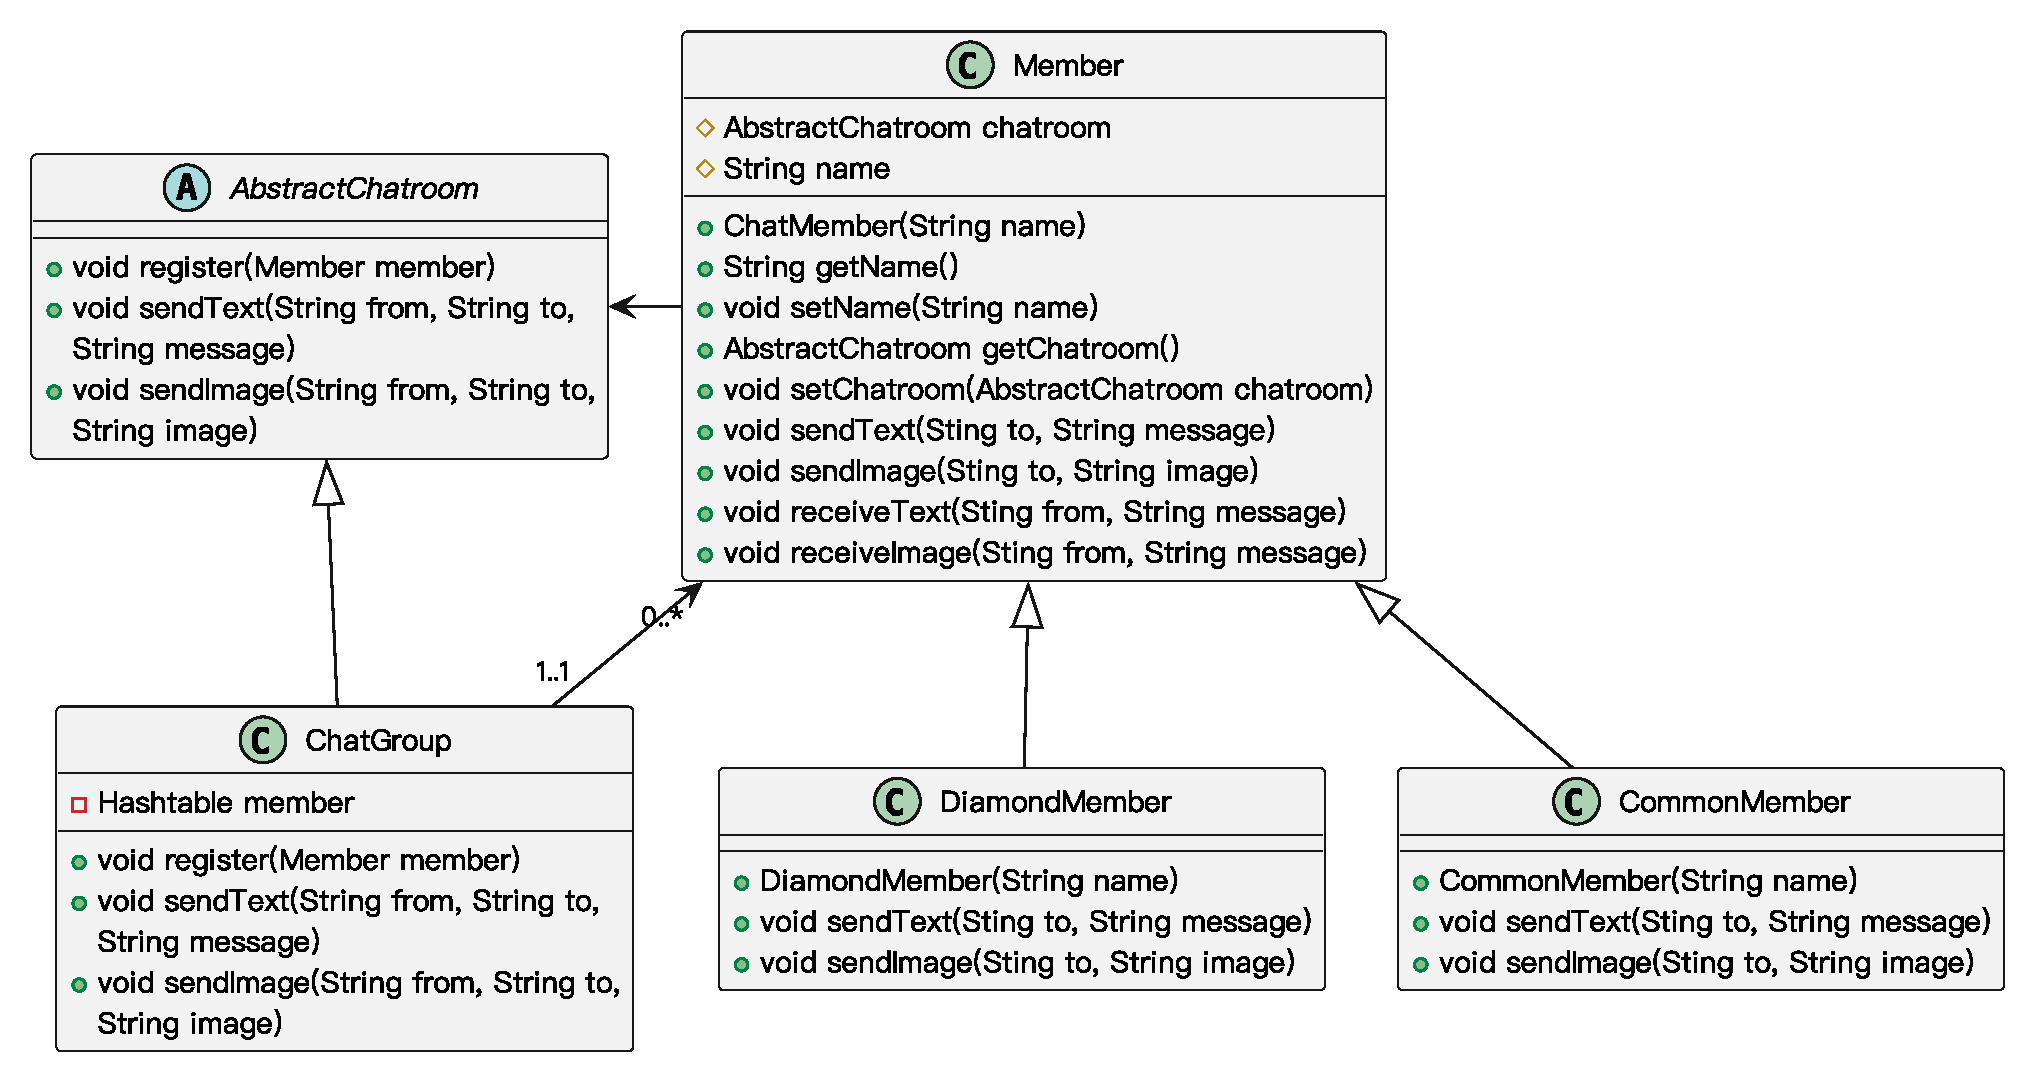
\includegraphics[width=0.95\textwidth]{images/中介者模式实例.eps}
    \vspace{-1em}
\end{figure}

\subsubsection{模式优缺点}
中介者模式的优点:
\vspace{-0.8em}
\begin{multicols}{2}
    \begin{itemize}
        \item 简化了对象之间的交互。
        \item 将各同事解耦。
        \item 减少子类生成。
        \item 可以简化各同事类的设计和实现。
    \end{itemize}
\end{multicols}
\vspace{-1em}

中介者模式的缺点:
\begin{itemize}
    \item 在具体中介者类中包含了同事之间的交互细节,可能会导致具体中介者类非常复杂,使得系统难以维护。
\end{itemize}

\subsubsection{模式适用环境}
在以下情况下可以使用中介者模式:
\begin{itemize}
    \item 系统中\textbf{对象之间存在复杂的引用关系},产生的相互依赖关系结构混乱且难以理解。
    \item 一个对象由于引用了其他很多对象并且直接和这些对象通信,导致\textbf{难以复用该对象}。
    \item \textbf{想通过一个中间类来封装多个类中的行为,而又不想生成太多的子类}。可以通过引入中介者类来实现,在中介者中定义对象交互的公共行为,如果需要改变行为则可以增加新的中介者类。
\end{itemize}

\subsubsection{模式应用}
\ding{172} 中介者模式在事件驱动类软件中应用比较多,在设计GUI应用程序时,组件之间可能存在较为复杂的交互关系,一个组件的改变将影响与之相关的其他组件,此时可以使用中介者模式来对组件进行协调。

\ding{173} MVC是Java EE的一个基本模式,此时控制器Controller作为一种中介者,它负责控制视图对象View和模型对象Model之间的交互。如在Struts中,Action就可以作为JSP页面与业务对象之间的中介者。

\subsubsection{模式扩展}
\paragraph*{中介者模式与迪米特法则}~{} \par
在中介者模式中,通过创造出一个中介者对象,\textbf{将系统中有关的对象所引用的其他对象数目减少到最少},使得一个对象与其同事之间的相互作用被这个对象与中介者对象之间的相互作用所取代。因此,\textbf{中介者模式就是迪米特法则的一个典型应用}。

\paragraph*{中介者模式与GUI开发}~{} \par
中介者模式可以方便地应用于图形界面(GUI)开发中,在比较复杂的界面中可能存在多个界面组件之间的交互关系。

对于这些复杂的交互关系,有时候我们可以引入一个中介者类,\textbf{将这些交互的组件作为具体的同事类,将它们之间的引用和控制关系交由中介者负责},在一定程度上简化系统的交互,这也是中介者模式的常见应用之一。


\subsection{模板方法模式}

\subsubsection{模式动机}
模板方法模式是\textbf{基于继承}的代码复用基本技术,模板方法模式的结构和用法也是面向对象设计的核心之一。在模板方法模式中,可以\textbf{将相同的代码放在父类中,而将不同的方法实现放在不同的子类中}。

在模板方法模式中,我们需要准备一个抽象类,将部分逻辑以具体方法以及具体构造函数的形式实现,然后声明一些抽象方法来让子类实现剩余的逻辑。不同的子类可以以不同的方式实现这些抽象方法,从而对剩余的逻辑有不同的实现,这就是模板方法模式的用意。模板方法模式体现了面向对象的诸多重要思想,是一种使用频率较高的模式。

\subsubsection{模式定义}
模板方法模式(Template Method Pattern):定义一个操作中算法的骨架,而将一些步骤延迟到子类中,模板方法使得子类可以不改变一个算法的结构即可重定义该算法的某些特定步骤。模板方法是一种类行为型模式。

\subsubsection{模式结构}
模板方法模式包含如下角色:
\vspace{-0.8em}
\begin{multicols}{2}
    \begin{itemize}
        \item AbstractClass:抽象类
        \item ConcreteClass:具体子类
    \end{itemize}
\end{multicols}
\vspace{-1em}

\begin{figure}[H]
    \vspace{-0.5em}
	\centering
	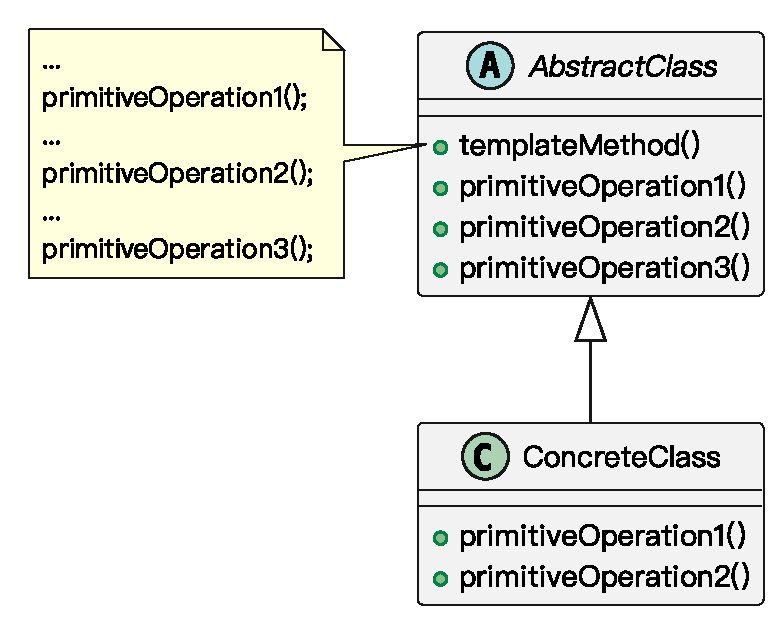
\includegraphics[width=0.45\textwidth]{images/模板方法模式结构.eps}
    \vspace{-1em}
\end{figure}

\subsubsection{模式分析}
模板方法模式是一种类的行为型模式,在它的结构图中\textbf{只有类之间的继承关系,没有对象关联关系}。

在模板方法模式的使用过程中,要求开发抽象类和开发具体子类的设计师之间进行协作。一个设计师负责\textbf{给出一个算法的轮廓和骨架},另一些设计师则负责\textbf{给出这个算法的各个逻辑步骤}。实现这些具体逻辑步骤的方法称为\textbf{基本方法}(Primitive Method),而将这些基本法方法汇总起来的方法称为\textbf{模板方法}(Template Method),模板方法模式的名字从此而来。
\begin{itemize}
    \item 模板方法:一个模板方法是定义在抽象类中的、把基本操作方法组合在一起形成一个总算法或一个总行为的方法。
    \item 基本方法:基本方法是实现算法各个步骤的方法,是模板方法的组成部分。
    \vspace{-0.8em}
    \begin{multicols}{3}
    \begin{itemize}
        \item 抽象方法
        \item 具体方法
        \item 钩子方法
    \end{itemize}
    \end{multicols}
    \vspace{-1em}
\end{itemize}
钩子方法(Hook Method):
\begin{lstlisting}
public void template(){
    open();
    display();
    if(isPrint()){
        print();
    }
}
public boolean isPrint(){
    return true;
}
\end{lstlisting}

模板方法模式典型代码:
\begin{figure}[H]
	\centering
	\includegraphics[width=\textwidth]{images/模板方法模式分析.pdf}
    \vspace{-2em}
\end{figure}

在模板方法模式中,由于面向对象的多态性,子类对象在运行时将覆盖父类对象,子类中定义的方法也将覆盖父类中定义的方法,因此程序在运行时,\textbf{具体子类的基本方法将覆盖父类中定义的基本方法,子类的钩子方法也将覆盖父类的钩子方法},从而可以通过在子类中实现的钩子方法对父类方法的执行进行约束,实现子类对父类行为的反向控制。

\subsubsection{模式实例}
银行业务办理流程:在银行办理业务时,一般都包含几个基本步骤,首先需要取号排队,然后办理具体业务,最后需要对银行工作人员进行评分。无论具体业务是取款、存款还是转账,其基本流程都一样。现使用模板方法模式模拟银行业务办理流程。
\begin{figure}[H]
    \vspace{-0.5em}
	\centering
	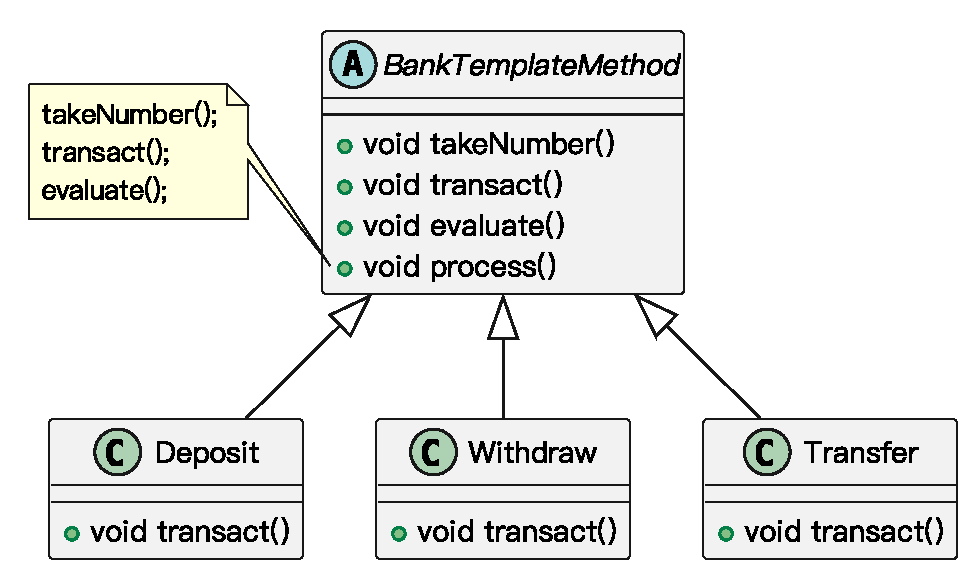
\includegraphics[width=0.55\textwidth]{images/模板方法模式实例1.eps}
    \vspace{-1em}
\end{figure}


数据库操作模板:对数据库的操作一般包括连接、打开、使用、关闭等步骤,在数据库操作模板类中我们定义了\sverb|connDB()|、\sverb|openDB()|、\sverb|useDB()|、\sverb|closeDB()|\;四个方法分别对应这四个步骤。对于不同类型的数据库(如SQL Server和Oracle),其操作步骤都一致,只是连接数据库\sverb|connDB()|\;方法有所区别,现使用模板方法模式对其进行设计。
\begin{figure}[H]
    \vspace{-0.5em}
	\centering
	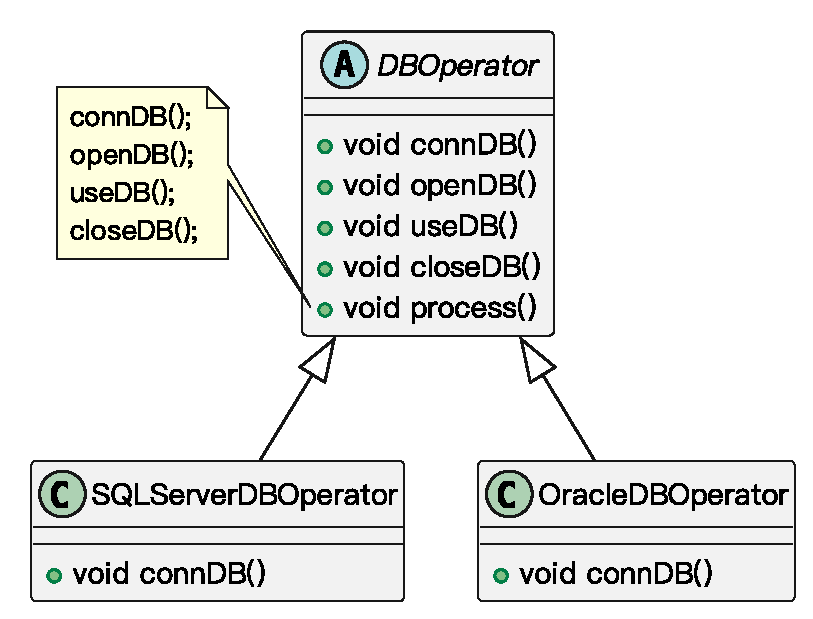
\includegraphics[width=0.5\textwidth]{images/模板方法模式实例2.eps}
    \vspace{-1em}
\end{figure}

\subsubsection{模式优缺点}
模板方法模式的优点:
\begin{itemize}
    \item 模板方法模式在一个类中抽象地定义算法,而由它的子类实现细节的处理。
    \item 模板方法模式是一种代码复用的基本技术。
    \item 模板方法模式导致一种反向的控制结构,通过一个父类调用其子类的操作,通过对子类的扩展增加新的行为,符合“开闭原则”。
\end{itemize}

模板方法模式的缺点:
\begin{itemize}
    \item 每个不同的实现都需要定义一个子类,这会导致类的个数增加,系统更加庞大,设计也更加抽象,但是更加符合“单一职责原则”,使得类的内聚性得以提高。
\end{itemize}

\subsubsection{模式适用环境}
在以下情况下可以使用模板方法模式:
\begin{itemize}
    \item 一次性实现一个算法的不变的部分,并将可变的行为留给子类来实现。
    \item 各子类中公共的行为应被提取出来并集中到一个公共父类中以避免代码重复。
    \item 对一些复杂的算法进行分割,将其算法中固定不变的部分设计为模板方法和父类具体方法,而一些可以改变的细节由其子类来实现。
    \item 控制子类的扩展。
\end{itemize}

\subsubsection{模式应用}
\ding{172} 模板方法模式广泛应用于框架设计(如Spring,Struts等)中,以确保父类控制处理流程的逻辑顺序(如框架的初始化)。

\ding{173} Java单元测试工具JUnit中的\sverb|TestCase|\;类的设计:
\begin{lstlisting}
...
public void runBare() throws Throwable {
    setUp();
    try {
        runTest(); 
    }finally { 
        tearDown();
    }
}
...
\end{lstlisting}

\subsubsection{模式扩展}

\paragraph*{关于继承的讨论}~{} \par
模板方法模式鼓励我们\textbf{恰当使用继承},此模式可以用来改写一些拥有相同功能的相关类,\textbf{将可复用的一般性的行为代码移到父类里面},而将特殊化的行为代码移到子类里面。这也进一步说明,虽然继承复用存在一些问题,但是在某些情况下还是可以给开发人员带来方便,\textbf{模板方法模式就是体现继承优势的模式之一}。

\paragraph*{好莱坞原则}~{} \par
在模板方法模式中,子类不显式调用父类的方法,而是通过覆盖父类的方法来实现某些具体的业务逻辑,父类控制对子类的调用,这种机制被称为好莱坞原则(Hollywood Principle),好莱坞原则的定义为:“不要给我们打电话,我们会给你打电话”。

在模板方法模式中,好莱坞原则体现在:\textbf{子类不需要调用父类,而通过父类来调用子类},将某些步骤的实现写在子类中,由父类来控制整个过程。

\paragraph*{钩子方法的使用}~{} \par
\begin{itemize}
    \item 钩子方法的引入使得子类可以控制父类的行为。
    \item 最简单的钩子方法就是空方法,也可以在钩子方法中定义一个默认的实现,如果子类不覆盖钩子方法,则执行父类的默认实现代码。
    \item 比较复杂一点的钩子方法可以对其他方法进行约束,这种钩子方法通常返回一个\sverb|boolean|\;类型,即返回\sverb|true|\;或\sverb|false|,用来判断是否执行某一个基本方法。
\end{itemize}

